\documentclass[ngerman,aspectratio=169,10pt]{beamer}

\usetheme[progressbar=frametitle]{metropolis}
\usepackage{appendixnumberbeamer}

\graphicspath{{./graphics/}}

\usepackage{booktabs}
\usepackage{xspace}
\usepackage{amsmath}
\usepackage{amssymb}
\usepackage{amsthm}
\usepackage{xfrac}
\usepackage{verbatim}
\usepackage{color}

\usepackage{stmaryrd}

\newcommand{\red}[1]{\textcolor{red}{#1}}
\newcommand{\grey}[1]{\textcolor{gray}{#1}}


\title{\vspace*{1.5em}A Block-Sorting Lossless Data Compression Algorithm}
\subtitle{\vspace*{-1.5em}}
% \date{16. November 2020}
\author{Finn Stutzenstein, Levin Nemesch, Joshua Sangmeister}
\institute{Algorithm Engineering - Übung 5}
\titlegraphic{
    \hfill
\includegraphics[height=1.5cm]{unilogo.pdf}\\
    \hspace*{8.3cm} \textsc{AG Theoretische Informatik}
}

\begin{document}

\maketitle

\begin{frame}{Kompression}
\begin{itemize}
    \item Ziel: Möglichst kurze Kodierung einer Information (z.B. Text)
    \item Bsp. \emph{Run-length encoding}: aaaabbbcaaa $\longrightarrow$ 4a3bc3a
    \item Problem: Finde gutes Kodierung. Viele Ansätze:
    \begin{itemize}
        \item 17\% e $\leftrightarrow$ 0,02\% q, ...
        \item Ein Buchstabe wird besonders häufig von einem anderen gefolgt
    \end{itemize}
    \item Hier: Ordne Text entsprechend neu an, sodass ähnliche Buchstaben zusammen stehen. Ermöglicht einfachere Kodierungen.
\end{itemize}
\end{frame}

\begin{frame}{Verfahren}
    Gegeben: Eingabealphabet $\Sigma$, Text $S\in \Sigma^*$, $N=|S|$
    \begin{enumerate}
        \item Transformation: $S\rightarrow(L, I)$, $L$ ist Permutation von $S$, $I\in\{0,\ldots,N-1\}$.
        \item Kompression von $(L, I)$ (Kein spezifisches Verfahren erforderlich)
        \item Dekompression von $(L, I)$
        \item Rücktransformation $(L, I)\rightarrow S$
    \end{enumerate}
\end{frame}

\begin{frame}{Transformation mit Beispiel}
    Beispieltext $S$ = 'abraca' ($N = 6$, $\Sigma=\{\text{'a'},\text{'b'},\text{'c'},\text{'r'}\}$)\\[1cm]
    
    Erstelle $N-1$ Rotationen (Leftshifts). Die erste Zeile ist $S$:\\
    \begin{tabular}{cccccc}
        \red{a}&\red{b}&\red{r}&\red{a}&\red{c}&\red{a}\vline\\
        b&r&a&c&a\vline&a\\
        r&a&c&a\vline&a&b\\
        a&c&a\vline&a&b&r\\
        c&a\vline&a&b&r&a\\
        a\vline&a&b&r&a&c\\
    \end{tabular}
\end{frame}

\begin{frame}{Transformation}
    Sortiere Rotationen lexikographisch in neue Matrix $M$:\\[20pt]
    
    \begin{tabular}{l|c c c c c c}
        &&&&&&$L$\\
        \hline
        0&a\vline&a&b&r&a&\textbf{c}\\
        \red{1}&\red{a}&\red{b}&\red{r}&\red{a}&\red{c}&\red{\textbf{a}}\vline\\
        2&a&c&a\vline&a&b&\textbf{r}\\
        3&b&r&a&c&a\vline&\textbf{a}\\
        4&c&a\vline&a&b&r&\textbf{a}\\
        5&r&a&c&a\vline&a&\textbf{b}\\
    \end{tabular}
    
    $I$ ist der Zeilenindex mit dem Originaltext.
    
    Ausgabe: $(L, I)$ (Im Beispiel $(\text{'caraab'}, 1)$)
\end{frame}

\begin{frame}{Wieso Preprocessing?}
	\begin{columns}
	    \begin{column}{0.46\textwidth}
	        $L$ ist sehr wahrscheinlich gut zu komprimieren. Mehrinformation durch $I$ vernachlässigbar.
	        \begin{itemize}
	            \item z.B. \textit{the} kommt sehr oft vor (englische Texte)
	            \item in $M$ dann viele Zeilen mit '$he\ldots t$' hintereinander
	            \item somit lange '$t$'-Folgen in $L$
	        \end{itemize}
	    \end{column}
	    \begin{column}{0.46\textwidth}
	        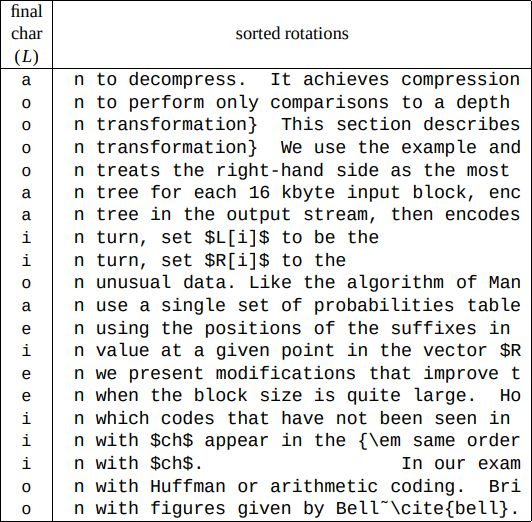
\includegraphics[width=200px]{graphics/table.jpg}
	    \end{column}
    \end{columns}
\end{frame}

\begin{frame}{Rücktransformation}
    Input: $(L, I)$ (hier: $(\text{'caraab'}, 1)$, insbesondere ist nicht die ganze Matrix verfügbar!)\\[5px]
    \begin{tabular}{l|c c c c c c}
        &F&&&&&$L$\\ \hline
        0&a\vline&a&b&r&a&\textbf{c}\\
        \red{1}&\red{a}&\red{b}&\red{r}&\red{a}&\red{c}&\red{\textbf{a}}\vline\\
        2&a&c&a\vline&a&b&\textbf{r}\\
        3&b&r&a&c&a\vline&\textbf{a}\\
        4&c&a\vline&a&b&r&\textbf{a}\\
        5&r&a&c&a\vline&a&\textbf{b}\\
    \end{tabular}
    \begin{itemize}
        \item Beobachtung: Jede Spalte ist Permutation von $S$
        \item Konstruiere $F$ durch Sortieren von $L$: $F$ = 'aaabcr'
    \end{itemize}
\end{frame}

\begin{frame}{Rücktransformation}
    \begin{columns}
        \begin{column}{0.46\textwidth}
            $M$:\\
            \begin{tabular}{l|c c c c c c}
                &$F$&&&&&$L$\\
                \hline
                0&\textbf{a}&a&b&r&a&c\\
                1&\textbf{a}&b&r&a&c&a\\
                2&\textbf{a}&c&a&a&b&r\\
                3&b&r&a&c&a&a\\
                4&c&a&a&b&r&a\\
                5&r&a&c&a&a&b\\
            \end{tabular}
        \end{column}
        \begin{column}{0.46\textwidth}
            $M'$ (einen Schritt nach rechts rotiert):
            \begin{tabular}{l|c c c c c c}
                &$L$&$F$&&&&\\ \hline
                0&c&a&a&b&r&a\\
                1&\textbf{a}&a&b&r&a&c\\
                2&r&a&c&a&a&b\\
                3&\textbf{a}&b&r&a&c&a\\
                4&\textbf{a}&c&a&a&b&r\\
                5&b&r&a&c&a&a\\
            \end{tabular}
        \end{column}
    \end{columns}
    \pause
    $M'$ ist lexikografisch nach dem \emph{zweiten} Zeichen sortiert
    
    $\longrightarrow$ Alle Zeilen, die mit dem selben Zeichen starten, sind in der selben Reihenfolge wie in $M$
    \pause
    
    $\longrightarrow$ Zuweisung der Einträge von $L$ auf $F$ (Zeilen von $M'$ auf $M$) mithilfe vom Vektor $T$
    \pause
    
    $\longrightarrow$ $T=(4, 0, 5, 1, 2, 3)$
\end{frame}

\begin{frame}{Rücktransformation}
    $L =$ ('c', 'a', 'r', 'a', 'a', 'b') \\
    $I=1$\\
    $T=(4, 0, 5, 1, 2, 3)$\\[7px]
    $M$:\\
    \begin{tabular}{l|c c c c c c}
        &$F$&&&&&$L$\\
        \hline
        0&a&a&b&r&a&c\\
        1&a&b&r&a&c&a\\
        2&a&c&a&a&b&r\\
        3&b&r&a&c&a&a\\
        4&c&a&a&b&r&a\\
        5&r&a&c&a&a&b\\
    \end{tabular}
\end{frame}

\begin{frame}{Suffix Arrays}
    Implementationsdetails:
    \begin{itemize}
        \item Rücktransformation ist einfach umsetzbar ($\mathcal{O}(N \log N)$, Sortierung von $L$)
        \item Transformation: Wie kann $\mathcal{O}(N^2 \log N)$ vermieden werden?
    \end{itemize}
    \pause
    
    Beobachtung: Rotation schiebt Suffixes nach vorne
    
    \begin{tabular}{cccccc}
        \red{a}&\red{b}&\red{r}&\red{a}&\red{c}&\red{a}\vline\\
        \red{b}&\red{r}&\red{a}&\red{c}&\red{a}\vline&a\\
        \red{r}&\red{a}&\red{c}&\red{a}\vline&a&b\\
        \red{a}&\red{c}&\red{a}\vline&a&b&r\\
        \red{c}&\red{a}\vline&a&b&r&a\\
        \red{a}\vline&a&b&r&a&c\\
    \end{tabular}
    
    \begin{itemize}
        \item Kann Suffix-Sorting statt String-Sorting verwendet werden?
    \end{itemize}
\end{frame}


\begin{frame}{Suffix Arrays}
    
    Hänge an $S$ ein extra Zeichen an, das nur dort vorkommt und minimal sortiert z.B. \$ 
    
    \begin{itemize}
        \item Beim ersten Vorkommen von \$ ist lexikographischer Vergleich eindeutig
    \end{itemize}
    
    \begin{columns}
	    \begin{column}{0.46\textwidth}
	        \begin{tabular}{ccccccc}
	            a&b&r&a&c&a&\$\\
	            b&r&a&c&a&\$&\\
	            r&a&c&a&\$&&\\
	            a&c&a&\$&&&\\
	            c&a&\$&&&&\\
	            a&\$&&&&&\\
	        \end{tabular}
	    \end{column}
	    \begin{column}{0.46\textwidth}
	        \begin{tabular}{ccccccc}
	            a&\$&&&&&\grey{c}\\
	            a&b&r&a&c&a&\$\\
	            a&c&a&\$&&&\grey{r}\\
	            b&r&a&c&a&\$&\grey{a}\\
	            c&a&\$&&&&\grey{a}\\
	            r&a&c&a&\$&&\grey{b}\\
	        \end{tabular}
	    \end{column}
    \end{columns}
\end{frame}

\begin{frame}{Suffix Sorting}
    \begin{itemize}
        \item Benutze Suffix-Arrays
        \item Sortieren in $\mathcal{O}(N)$
        \item Suffix-Array speichert $F$
        \item Für $L$ einfache modulo Operation
    \end{itemize}
\end{frame}

\end{document}